% 옛 그림 2의 패널 (b). 저자가 직접 그린 StandAlone 어텐션 한 지점
% (images/Frequency_Adapataion.pdf 7쪽).
\begin{figure}[t]
\centering
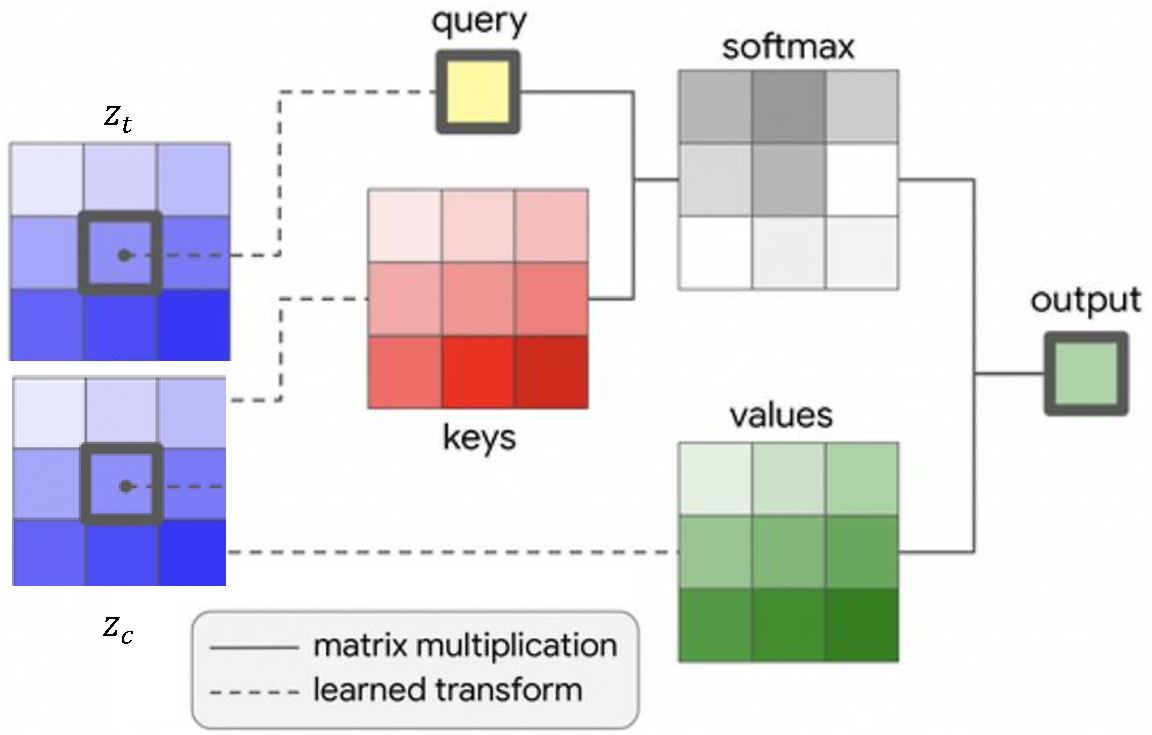
\includegraphics[width=\columnwidth]{figures/sa_adapter}
\caption{StandAlone 한 지점. 쿼리는 UNet latent $z_t$의 한 위치이고, 키와 값은 조건
$z_c$에서 같은 위치의 $3{\times}3$ 이웃이다. 따라서 softmax는 전체 맵이 아니라 9개에
대해 계산되며, $1{\times}1$ 창도 적어도 그만큼 잘 작동한다(\ref{sec:where}절). $W_K$,
$W_V$와 0초기화 채널별 게이트가 학습되고 $W_Q$와 출력 투영은 동결이다. 게이트를 지난
결과는 latent에 더해져 아래의 텍스트 쿼리가 구조를 보게 하고, 층이 반환하는 값에도
더해진다.}
\label{fig:sa}
\end{figure}
